\chapter{Projekt serwisu}
\thispagestyle{chapterBeginStyle}

W tym rozdziale przedstawiono szczegółowy projekt systemu w notacji UML uwzględniający wymagania funkcjonalne opisane w rozdziale~\ref{rozdzial1}. Do opisu relacji pomiędzy składowymi systemu wykorzystano diagramy \ldots.

\section{Założenia}

W serwisie wykorzystano architekturę klient-serwer. Istnieje jeden serwer, do którego może podłączać się wiele klientów i odpowiada on za komunikację i zarządzanie danymi.
W komponencie klienta wykorzystano architekturę trójwarstwową. Architektura ta dzieli komponent na trzy osobne części:
\begin{itemize}
	\item warstwa prezentacji,
	\item warstwa biznesowa,
	\item warstwa danych.
\end{itemize}
Warstwa prezentacji jest to interfejs graficzny użytkownika. Jest odpowiedzialna za interakcję z użytkownikiem (wyświetlanie i wprowadzanie danych). \\ \\
Warstwa biznesowa odpowiada za przetwarzanie komunikatów od użytkownika lub ze strony serwera. Tutaj zawarta jest wszelka logika aplikacji. Przetworzone dane są przekazywane do warstwy prezentacji i/lub warstwy danych. Warstwa ta jest łącznikiem pomiędzy warstwą prezentacji, a warstwą danych. \\ \\
Warstwa danych jest dostępem do danych. Obsługuje połączenie aplikacji z zewnętrznym obiektem dostarczającym dane (baza danych, serwer).

\section{Przypadki użycia i scenariusze}

W tej sekcji należy przedstawić przypadki użycia oraz odpowiadające im scenariusze dla poszczególnych grup użytkowników \ldots.

\section{Diagramy klas}

W tej sekcji należy przedstawić diagramy klas dla odpowiednich elementów systemu zidentyfikowane na podstawie wcześniejszych rozważań 

\section{Diagramy aktywności}

W tej sekcji należy przedstawić diagramy aktywności dla elementów systemu i odpowiednich procesów wynikające z wcześniejszej analizy.  

{\color{dgray}
W niniejszym rozdziale przedstawiono diagramy aktywności \ldots. Diagram na rysunku~\ref{czynnosci_GD} przedstawia \ldots.
} 

\begin{figure}[h!]
\begin{center}
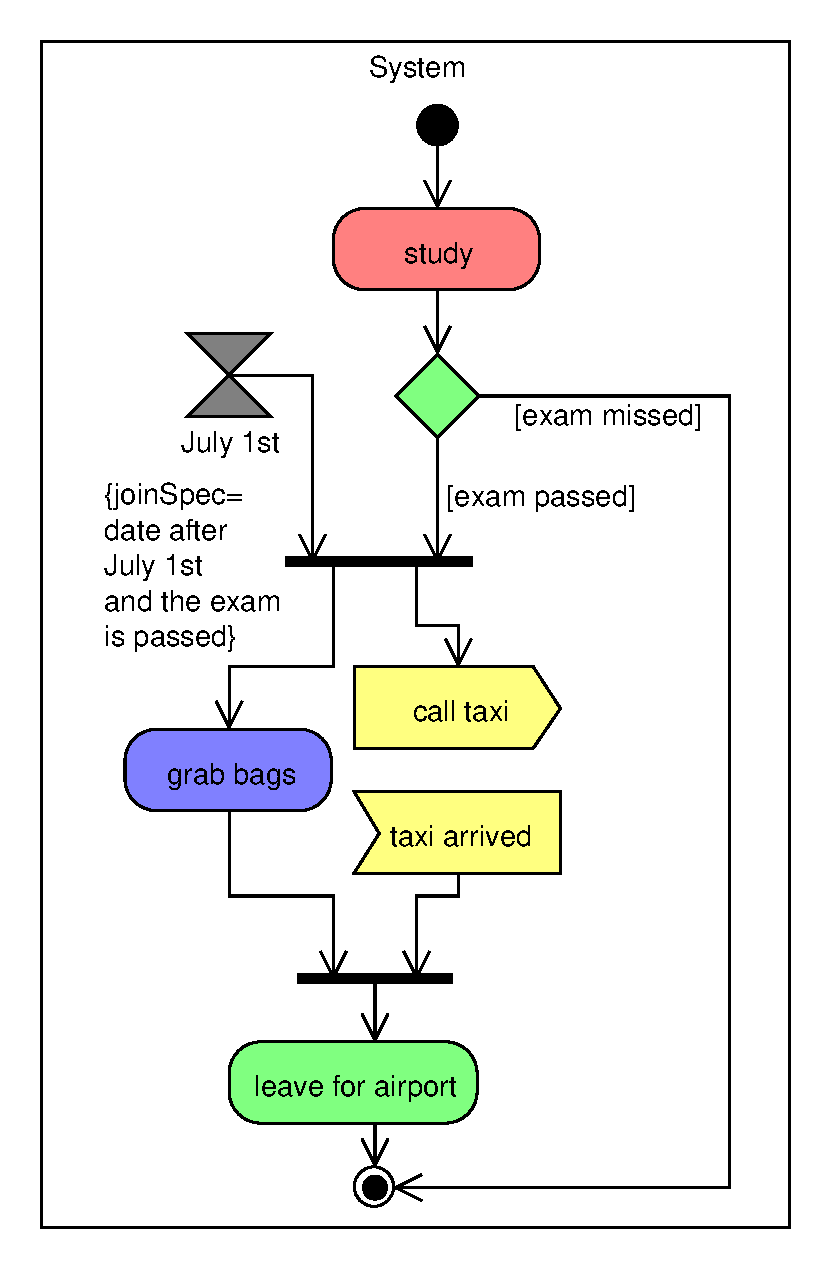
\includegraphics[width=0.5\textwidth]{aktyw.pdf}
\end{center}
\caption{{\color{dgray}Diagram aktywności związany z procesem rejestracji dokumentu.}} \label{czynnosci_GD}
\end{figure}  

\section{Diagramy sekwencji}

W tej sekcji należy przedstawić diagramy sekwencji dla obiektów systemu zidentyfikowanych na podstawie wcześniejszych rozważań. Należy wykorzystać nazewnictwo wprowadzone w poprzednich rozdziałach, w szczególności odpowiadające definicjom wprowadzonych klas.

\section{Diagramy stanów}

W tej sekcji należy przedstawić diagramy stanów w których może znaleźć się system. Diagramy te są szczególnie istotne przy projektowaniu systemów czasu rzeczywistego. 

\section{Projekt bazy danych}

W tej sekcji należy przedstawić projekt bazy danych. Należy omówić wycinek rzeczywistości i odpowiadające mu zidentyfikowane elementy systemu, których wartości będą podlegać utrwalaniu. Należy przedyskutować wybór typów danych dla atrybutów poszczególnych obiektów. Należy uzasadnić wybór platformy DBMS. Dla relacyjnych baz danych należy przedyskutować jej normalizację.

\section{Opis protokołów}

W tej sekcji należy omówić protokoły wykorzystywane przez komponenty systemu. Omówić formaty komunikatów i zilustrować je przykładami. 

\section{Opis algorytmów}

W tej sekcji należy wymienić i przedyskutować algorytmy wykorzystywane w systemie. Algorytmy należy przedstawić w pseudokodzie (wykorzystać pakiet \texttt{algorithm2e}). Omówienia poszczególnych kroków algorytmów powinny zawierać odwołania do odpowiednich linii pseudokodu. Dla zaproponowanych autorskich algorytmów należy przeprowadzić analizę ich złożoności czasowej i pamięciowej. 

{\color{dgray}
Algorytm bąblowania jest przedstawiony w Pseudokodzie~\ref{alg:mine}.
}

{\small
\begin{pseudokod}[H]
%\SetAlTitleFnt{small}
\SetArgSty{normalfont}
\SetKwFunction{Process}{Process}
\SetKwFunction{Calculate}{Calculate}
\KwIn{Zbiór bąbli $B$}
\KwOut{Wyporność $W$}
\ForEach{$b \in B$}{
\Process{$b$}\;
\For{$i \leftarrow 1$ \KwTo $|B|$}{
\If{\Calculate{EW($i$,$b$)} $\le$ 0}{
$b \leftarrow 2*b$\;
}
}
}
\While{$B \neq \emptyset$}{
\For{$j \leftarrow 1$ \KwTo $|B|$}{
\If{\Calculate{FT($j$,$\hat{b}$)} $\le 0$}{
$w \leftarrow 2*\hat{b}$\;
$W \leftarrow W \cup \{w\}$\;
$B \leftarrow B \setminus \{b\}$\;
}
}
}
\caption{Wyporność przez bąblowanie}\label{alg:mine}
\end{pseudokod}
}

